%
% fe.tex -- finite elemente
%
% (c) 2018 Prof Dr Andreas Müller, Hochschule Rapperswil
%
\documentclass[tikz]{standalone}
\usepackage{times}
\usepackage{txfonts}
\usepackage[utf8]{inputenc}
\usepackage{graphics}
\usepackage{ifthen}
\usepackage{color}
\usetikzlibrary{arrows,intersections}
\begin{document}


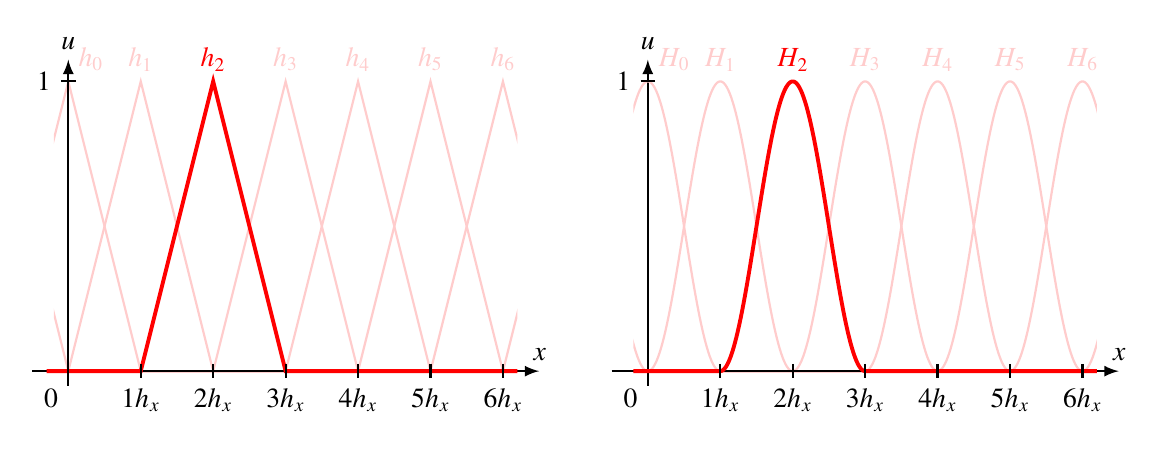
\begin{tikzpicture}[thick,>=latex,scale=0.92]

\begin{scope}[xshift=-4cm]


\begin{scope}
\clip (-0.2,-0.1) rectangle (6.2,4.1);
\draw[color=red!20] (-3,0)--(-2,4)--(-1,0)--(6,0);
\draw[color=red!20] (-2,0)--(-1,4)--(0,0)--(6,0);
\draw[color=red!20] (-1,0)--(0,4)--(1,0)--(6,0);
\draw[color=red!20] (-0.3,0)--(0,0)--(1,4)--(2,0)--(6,0);
\draw[color=red!20] (-0.3,0)--(2,0)--(3,4)--(4,0)--(6,0);
\draw[color=red!20] (-0.3,0)--(3,0)--(4,4)--(5,0)--(6,0);
\draw[color=red!20] (-0.3,0)--(4,0)--(5,4)--(6,0)--(6,0);
\draw[color=red!20] (-0.3,0)--(5,0)--(6,4)--(7,0);
\draw[color=red!20] (-0.3,0)--(6,0)--(7,4)--(8,0);
\end{scope}

\draw[->] (-0.5,0)--(6.5,0) coordinate[label={above:$x$}];

\draw[color=red,line width=1.4pt] (-0.3,0)--(1,0)--(2,4)--(3,0)--(6.2,0);

\draw[->] (0,-0.2)--(0,4.3) coordinate[label={above:$u$}];

\node[color=red!20] at (0,4) [above right] {$h_0$};
\node[color=red!20] at (1,4) [above] {$h_1$};
\node[color=red] at (2,4) [above] {$h_2$};
\node[color=red!20] at (3,4) [above] {$h_3$};
\node[color=red!20] at (4,4) [above] {$h_4$};
\node[color=red!20] at (5,4) [above] {$h_5$};
\node[color=red!20] at (6,4) [above] {$h_6$};

\draw (-0.1,4)--(0.1,4);
\node at (-0.1,4) [left] {$1$};
\node at (0,-0.1) [below left] {$0$};

\foreach \x in {1,2,...,6}{
\draw ({\x},0.1)--({\x},-0.1);
\node at ({\x},-0.1) [below] {${\x}h_x$};
}
\end{scope}

\begin{scope}[xshift=4cm]

\draw[->] (0,-0.2)--(0,4.3) coordinate[label={above:$u$}];

\begin{scope}
\clip (-0.2,-0.1) rectangle (6.2,4.1);

\begin{scope}[xshift=-1cm]
\draw[color=red!20] (-5,0)--
	plot[domain=-180:180,samples=100] ({\x/180},{2 + 2*cos(\x)})
	-- (5,0);
\end{scope}
\begin{scope}[xshift=0cm]
\draw[color=red!20] (-5,0)--
	plot[domain=-180:180,samples=100] ({\x/180},{2 + 2*cos(\x)})
	-- (5,0);
\end{scope}
\begin{scope}[xshift=1cm]
\draw[color=red!20] (-5,0)--
	plot[domain=-180:180,samples=100] ({\x/180},{2 + 2*cos(\x)})
	-- (5,0);
\end{scope}
\begin{scope}[xshift=3cm]
\draw[color=red!20] (-5,0)--
	plot[domain=-180:180,samples=100] ({\x/180},{2 + 2*cos(\x)})
	-- (5,0);
\end{scope}
\begin{scope}[xshift=4cm]
\draw[color=red!20] (-5,0)--
	plot[domain=-180:180,samples=100] ({\x/180},{2 + 2*cos(\x)})
	-- (5,0);
\end{scope}
\begin{scope}[xshift=5cm]
\draw[color=red!20] (-5,0)--
	plot[domain=-180:180,samples=100] ({\x/180},{2 + 2*cos(\x)})
	-- (5,0);
\end{scope}
\begin{scope}[xshift=6cm]
\draw[color=red!20] (-5,0)--
	plot[domain=-180:180,samples=100] ({\x/180},{2 + 2*cos(\x)})
	-- (5,0);
\end{scope}
\begin{scope}[xshift=7cm]
\draw[color=red!20] (-5,0)--
	plot[domain=-180:180,samples=100] ({\x/180},{2 + 2*cos(\x)})
	-- (5,0);
\end{scope}
\end{scope}

\draw[->] (-0.5,0)--(6.5,0) coordinate[label={above:$x$}];

\begin{scope}
\clip (-0.2,-0.1) rectangle (6.2,4.1);
\begin{scope}[xshift=2cm]
\draw[color=red,line width=1.4pt] (-5,0)--
	plot[domain=-180:180,samples=100] ({\x/180},{2 + 2*cos(\x)})
	-- (5,0);
\end{scope}

\end{scope}

\node[color=red!20] at (0,4) [above right] {$H_0$};
\node[color=red!20] at (1,4) [above] {$H_1$};
\node[color=red] at (2,4) [above] {$H_2$};
\node[color=red!20] at (3,4) [above] {$H_3$};
\node[color=red!20] at (4,4) [above] {$H_4$};
\node[color=red!20] at (5,4) [above] {$H_5$};
\node[color=red!20] at (6,4) [above] {$H_6$};

\draw (-0.1,4)--(0.1,4);
\node at (-0.1,4) [left] {$1$};
\node at (0,-0.1) [below left] {$0$};

\foreach \x in {1,2,...,6}{
\draw ({\x},0.1)--({\x},-0.1);
\node at ({\x},-0.1) [below] {${\x}h_x$};
}
\end{scope}

\end{tikzpicture}

\end{document}
